\documentclass[12pt]{beamer}
\usepackage[utf8]{inputenc}
%\usepackage[latin1]{inputenc}
\usepackage[spanish]{babel}
%\usetheme{Warsaw}
%\usepackage{euler}
\usepackage{amsmath}
\usepackage{amsthm}
\usepackage{multicol}
\usepackage{multirow}
\usepackage{graphicx}
\usepackage{tikz}
\usepackage{color}
\usepackage{listings}
\renewcommand*{\multirowsetup}{\centering}
\lstset{ %
language=Python,                % choose the language of the code
basicstyle=\footnotesize,       % the size of the fonts that are used for the code
numbers=left,                   % where to put the line-numbers
numberstyle=\footnotesize,      % the size of the fonts that are used for the line-numbers
stepnumber=1,                   % the step between two line-numbers. If it is 1 each line will be numbered
numbersep=5pt,                  % how far the line-numbers are from the code
backgroundcolor=\color{white},  % choose the background color. You must add \usepackage{color}
showspaces=false,               % show spaces adding particular underscores
showstringspaces=false,         % underline spaces within strings
showtabs=false,                 % show tabs within strings adding particular underscores
frame=single,   		% adds a frame around the code
tabsize=4,  		% sets default tabsize to 2 spaces
captionpos=b,   		% sets the caption-position to bottom
breaklines=true,    	% sets automatic line breaking
breakatwhitespace=false,    % sets if automatic breaks should only happen at whitespace
escapeinside={\%}{)}          % if you want to add a comment within your code
}
%\usepackage{epstopdf}
\DeclareGraphicsExtensions{.pdf,.png,.jpg}
\renewcommand {\arraystretch}{1.5}
\mode<presentation>
{
  \usetheme{Warsaw}
  \setbeamercovered{transparent}
  % or whatever (possibly just delete it)
}
\title{Tema 1 - Material de apoyo}
\subtitle{Curso de F\'{i}sica Computacional}
\author{M. en C. Gustavo Contreras May\'{e}n}
%\email{curso.fisica.comp@gmail.com}
%\ptsize{10}
\begin{document}
\maketitle
\fontsize{14}{14}\selectfont
\spanishdecimal{.}
\begin{frame}{Contenido}
\tableofcontents[pausesections]
\end{frame}
\section{¿Para qu\'{e} Numpy?}
\begin{frame}
\frametitle{¿Para qu\'{e} Numpy?}
El objeto principal de Numpy es el arreglo multidimensional homog\'{e}neo. Es una tabla de elementos (normalmente n\'{u}meros ) donde todos ellos son del mismo tipo, indizados por una tupla de enteros positivos. En Numpy las \textit{dimensiones} son llamadas \textcolor{red}{ejes}. Al n\'{u}mero de ejes se llama \textcolor{blue}{rango}.
\\
\bigskip
Por ejemplo, las coordenadas de un punto en el espacio 3D $[1,2,1]$ es un arreglo de rango 1, ya que tiene s\'{o}lo un eje. Ese eje tiene una longitud de 3.
\end{frame}
\begin{frame}
\[ \begin{split}
[[1., 0., 0.], \\
[0., 1., 2. ]]
\end{split} \]
El arreglo es de rango 2 (por que es de dimensi\'{o}n 2), la primera dimensi\'{o}n (o eje) tiene una longitud de 2, la segunda dimensi\'{o}n tiene longitud 3.
\\
\bigskip
La clase en Numpy para arreglos es \texttt{ndarray}, que tambi\'{e}n es conocido con el alias de \texttt{array}. N\'{o}tese que \texttt{numpy.array} no es el mismo elemento de la librer\'{i}a est\'{a}ndar de Python \texttt{array.array}, ya que \'{e}sta s\'{o}lo maneja arreglos de 1D y ofrece menos funcionalidad.
\end{frame}
\subsection{Atributos de \texttt{ndarray}.}
\begin{frame}
\frametitle{Atributos de \texttt{ndarray}}
Los atributos m\'{a}s importantes de un objeto \texttt{ndarray} son:
\begin{itemize}
\item \textbf{ndarray.dim}: es el n\'{u}mero de ejes en el arreglo. En el Universo Python, el n\'{u}mero de dimensiones se conoce como \textit{rango}.
\item \textbf{ndarray.shape}: son las dimensiones del arreglo. Es una tupla de enteros que indican el tamaño del arreglo en cada dimensi\'{o}n. Para un arreglo (matriz) con $n$ renglones y $m$ columnas, \texttt{shape} ser\'{a} \texttt{(n,m)}. La longitud de la tupla \texttt{shape}, es por tanto el rango, o n\'{u}mero de dimensiones, \texttt{ndim}.
\end{itemize}
\end{frame}
\begin{frame}
\frametitle{Atributos de \texttt{ndarray}}
\begin{itemize}
\item \textbf{ndarray.size}: es el total de n\'{u}mero de elementos en el arreglo. Es igual al producto de los elementos de \texttt{shape}.
\item \textbf{ndarray.dtype}: es un objeto que describe el tipo de elementos en el arreglo. Podemos crear un d-tipeado espec\'{i}fico, usando los tipos est\'{a}ndar de Python; Numpy proporciona tipos propios: \texttt{numpy.int32}, \texttt{numpy.int16} y \texttt{numpy.float64} como ejemplos.
\end{itemize}
\end{frame}
\begin{frame}[fragile]
\frametitle{Ejemplos 1}
\texttt{>>> from numpy import *} \\
\visible<2->{\texttt{>>> a = arange(15).reshape(3,5)}} \\
\visible<3->{\texttt{>>> a}} \\
\visible<4->{\textcolor{blue}{\texttt{array ([[0,1,2,3,4],}}} \\
\visible<4->{\hspace{1cm} \textcolor{blue}{[5, 6, 7, 8, 9],}} \\
\visible<4->{\hspace{1cm} \textcolor{blue}{[10, 11, 12, 13, 14]])}} \\
\visible<5->{\texttt{>>> a.shape}}\\
\visible<6->{\textcolor{blue}{\texttt{(3,5)}}}\\
\visible<7->{\texttt{>>> a.ndim}}\\
\visible<8->{\textcolor{blue}{\texttt{2}}}\\
\visible<9->{\texttt{>>> a.dtype.name}}\\
\visible<10->{\textcolor{blue}{\texttt{'int32'}}}\\
\visible<11->{\texttt{>>> a.itemsize}}\\
\visible<12->{\textcolor{blue}{\texttt{4}}}\\
\end{frame}
\begin{frame}[fragile]
\frametitle{Ejemplos 2}
\texttt{>>> a.size} \\
\visible<2->{\textcolor{blue}{\texttt{15}}} \\
\visible<3->{\texttt{>>> type(a)}} \\
\visible<4->{\textcolor{blue}{\texttt{numpy.ndarray}}} \\
\visible<5->{\texttt{>>> b = array([6,7,8])}} \\
\visible<6->{\texttt{>>> b}} \\
\visible<7->{\textcolor{blue}{\texttt{array ([6,7,8])}}} \\
\visible<8->{\texttt{>>> type(b)}} \\
\visible<9->{\textcolor{blue}{\texttt{numpy.ndarray}}} \\
\end{frame}
\section{Creando un arreglo}
\begin{frame}[fragile]
\frametitle{Creando un arreglo}
Existen diversas maneras para crear los arreglos.
\\
\bigskip
Por ejemplo, podemos crear un arreglo de una lista o tupla regular de Python, usando la funci\'{o}n \texttt{array}. El tipo de de arreglo resultante se deduce del tipo de elementos en la secuencia.
\\
\medskip
\texttt{>>> from numpy import *} \\
\visible<2->{\texttt{>>> a = array([2,3,4])}} \\
\visible<3->{\texttt{>>> a}}\\
\visible<4->{\textcolor{blue}{\texttt{array([2,3,4])}}}\\
\visible<5->{\texttt{>>> a.dtype}} \\
\visible<6->{\textcolor{blue}{\texttt{dtype('int32')}}} \\
\visible<7->{\texttt{>>> b = array ([1.2, 3.5, 5.1])}} \\
\visible<8->{\texttt{>>> b.dtype}} \\
\visible<9->{\textcolor{blue}{\texttt{'float64'}}} \\
\end{frame}
\begin{frame}
\frametitle{Precauci\'{o}n}
Un error que se presenta frecuentemente es llamar a la funci\'{o}n \texttt{array} con m\'{u}ltiples argumentos, en lugar de proporcionar una  \'{u}nica lista de n\'{u}meros.
\\
\bigskip
\visible<2->{\texttt{>>> a = array (1,2,3,4)} \hspace{2cm} \textcolor{red}{Mal hecho}} \\
\visible<3->{\texttt{>>> a = array ([1,2,3,4])} \hspace{1.5cm} \textcolor{blue}{Bien hecho}} \\
\end{frame}
\begin{frame}
A menudo, los elementos de un arreglo no se conocen desde el inicio del problema, pero su tamaño si; Numpy proporciona algunas funciones que generan arreglos con un contenido inicial, con la finalidad de minimizar el crecimiento de arreglos, que es a su vez, una tarea que gasta recursos.
\\
\bigskip
\begin{enumerate}[<+->]
\item \texttt{zeros}: genera un arreglo donde todos los elementos son ceros.
\item \texttt{ones}: genera un arreglo donde todos los elementos del mismo son unos.
\item \texttt{empty:} genera un arreglo con valores iniciales aleatorios, por defecto, el tipo de dato es \texttt{float64}.
\end{enumerate}
\end{frame}
\begin{frame}
\texttt{>>> zeros((3,4))} \\
\visible<2->{\textcolor{blue}{\texttt{array([[0., 0., 0., 0.],}}} \\
\visible<2->{\textcolor{blue}{\hspace{1cm} \texttt{[0., 0., 0., 0.],}}} \\
\visible<2->{\textcolor{blue}{\hspace{1cm} \texttt{[0., 0., 0., 0.]])}}} \\
\visible<3->{ \texttt{>>> ones((2,3,4), dtype=int16)}} \\
\visible<4->{\textcolor{blue}{\texttt{array([[[1, 1, 1, 1],}}} \\
\visible<4->{\textcolor{blue}{\hspace{1cm} \texttt{[1, 1, 1, 1],}}} \\
\visible<4->{\textcolor{blue}{\hspace{1cm} \texttt{[1, 1, 1, 1]],}}} \\
\visible<4->{\textcolor{blue}{\hspace{1cm} \texttt{[[1, 1, 1, 1],}}} \\
\visible<4->{\textcolor{blue}{\hspace{1cm} \texttt{[1, 1, 1, 1],}}} \\
\visible<4->{\textcolor{blue}{\hspace{1cm} \texttt{[1, 1, 1, 1]]], dtype=int16)}}} \\
\visible<5->{ \texttt{>>> empty((2,3))}} \\
\end{frame}
\section{La funci\'{o}n \texttt{arange}}
\begin{frame}
\frametitle{La funci\'{o}n \texttt{arange}}
Para crear una secuencia de n\'{u}meros, Numpy cuenta con una funci\'{o}n  an\'{a}loga a \texttt{range}, que devuelve arreglos en lugar de listas.
\\
\bigskip
\texttt{>>> arange(10, 30, 5)} \\
\visible<2->{\textcolor{blue}{\texttt{([10, 15, 20, 25])}}} \\
\visible<3->{\texttt{>>> arange(0, 2, 0.3)}} \\
\visible<4->{\textcolor{blue}{\texttt{([0., 0.3, 0.6, 0.9, 1.2, 1.5, 1.8])}}}
\end{frame}
\section{Funci\'{o}n \texttt{linspace}}
\begin{frame}
\frametitle{Funci\'{o}n \texttt{linspace}}
Cuando \texttt{arange} se usa con argumentos de punto flotante, en general no es posible predecir el n\'{u}mero de elementos obtenidos, debido a la precisi\'{o}n de punto flotante. Por tanto, es mejor usar la funci\'{o}n \texttt{linspace}, en el argumento de la funci\'{o}n, se indica el n\'{u}mero de elementos que queremos, en vez de un paso.
\\
\bigskip
\texttt{>>> linspace(0,2,9)} \\
\visible<2->{\textcolor{blue}{\texttt{array([0., 0.25, 0.5, 0.75, 1., 1.25, 1.5, 1.75, 2.])}}} \\
\visible<3->{\texttt{>>> x = linspace(0,2*pi, 100)}} \\
\visible<4->{\texttt{>>> f = sin(x)}} \\
\end{frame}
\section{Graficando datos}
\begin{frame}
\frametitle{Graficando datos}
En el curso tendremos la necesidad de graficar datos obtenidos a partir de una aproximaci\'{o}n num\'{e}rica, para ello, usaremos \texttt{matplotlib} que es un m\'{o}dulo de Python con el que tendremos la oportunidad de elaborar gr\'{a}ficas desde b\'{a}sicas hasta unas m\'{a}s elaboradas.
\\
\bigskip
Como hemos mencionado, ya un abordaje m\'{a}s profundo en este m\'{o}dulo requiere de tiempo que tendr\'{a}n que dedicarle por su cuenta.
\end{frame}
\begin{frame}[fragile]
\frametitle{Ejemplo 1}
%\begin{minipage}[h]{5cm}
\begin{lstlisting}
import matplotlib.pyplot as plt
plt.plot([1,2,3,4])
plt.ylabel('algunos valores')
plt.show()
\end{lstlisting}
%\end{minipage}
\hspace{0.5cm}
\visible<2->{
\begin{minipage}[h]{0.9\textwidth}
\begin{figure}
	\centering	
	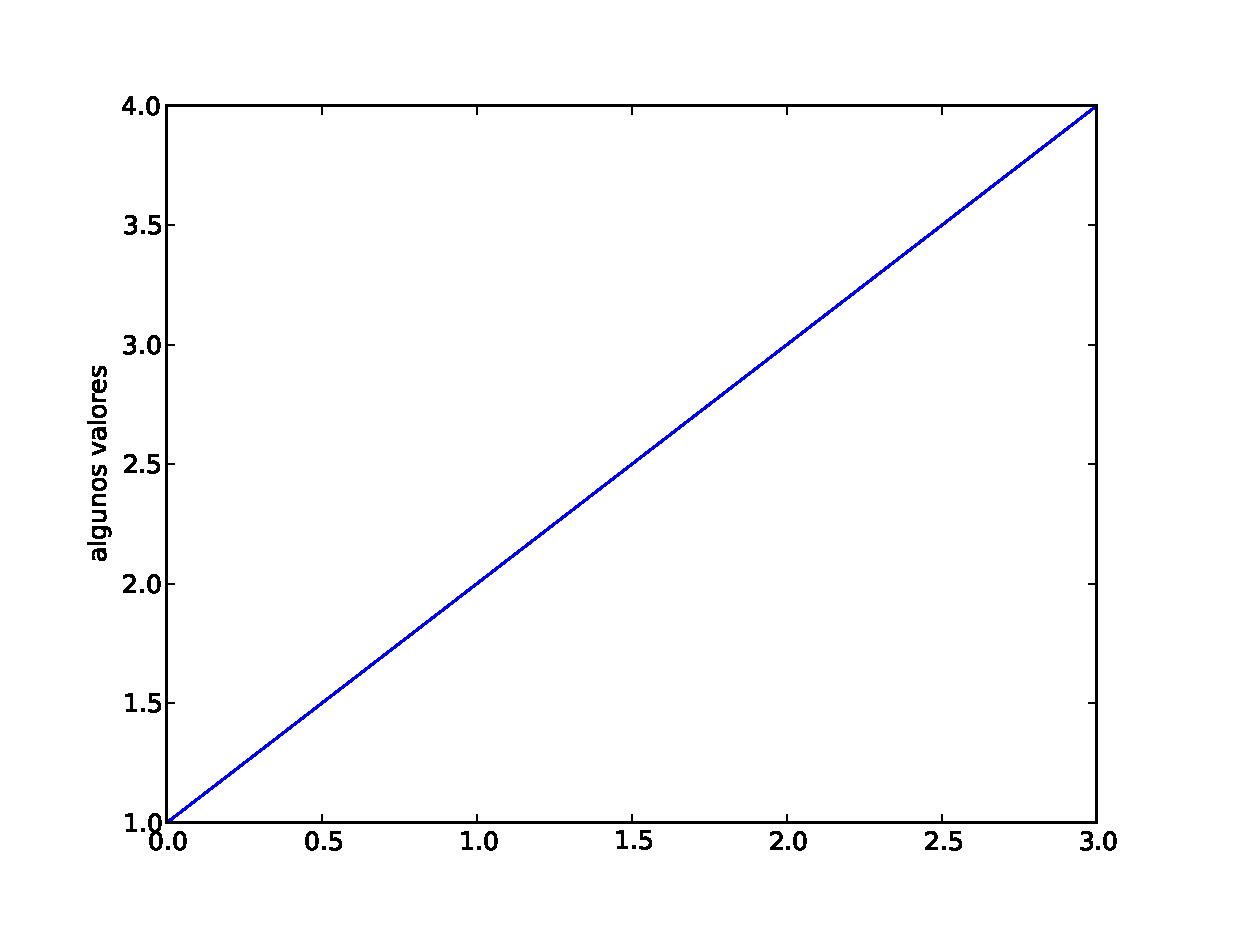
\includegraphics[scale=0.3]{ejemgraf1.eps} 
\end{figure}
\end{minipage}}
\end{frame}
\begin{frame}[fragile]
\frametitle{Ejemplo 2}
\begin{lstlisting}
import matplotlib.pyplot as plt
plt.plot([1,2,3,4],[1,4,9,16])
plt.show()
\end{lstlisting}
\hspace{0.5cm}
\visible<2->{
\begin{minipage}[h]{0.9\textwidth}
\begin{figure}
	\centering	
	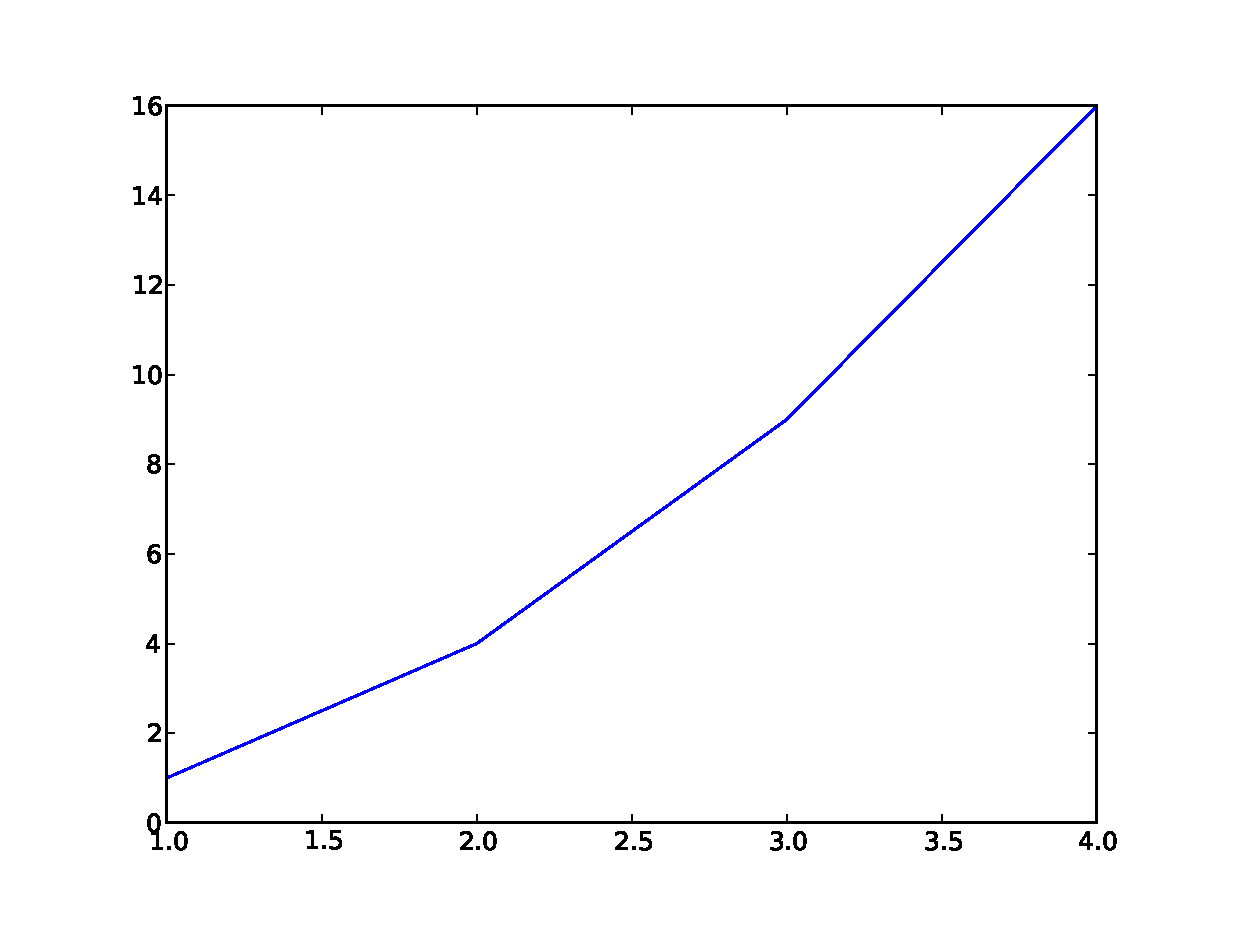
\includegraphics[scale=0.3]{ejemgraf2.eps} 
\end{figure}
\end{minipage}}
\end{frame}
\begin{frame}[fragile]
\frametitle{Ejemplo 3}
\begin{lstlisting}
import matplotlib.pyplot as plt
plt.plot([1,2,3,4], [1,4,9,16], 'ro')
plt.axis([0, 6, 0, 20])
plt.show()
\end{lstlisting}
\hspace{0.5cm}
\visible<2->{
\begin{minipage}[h]{0.9\textwidth}
\begin{figure}
	\centering	
	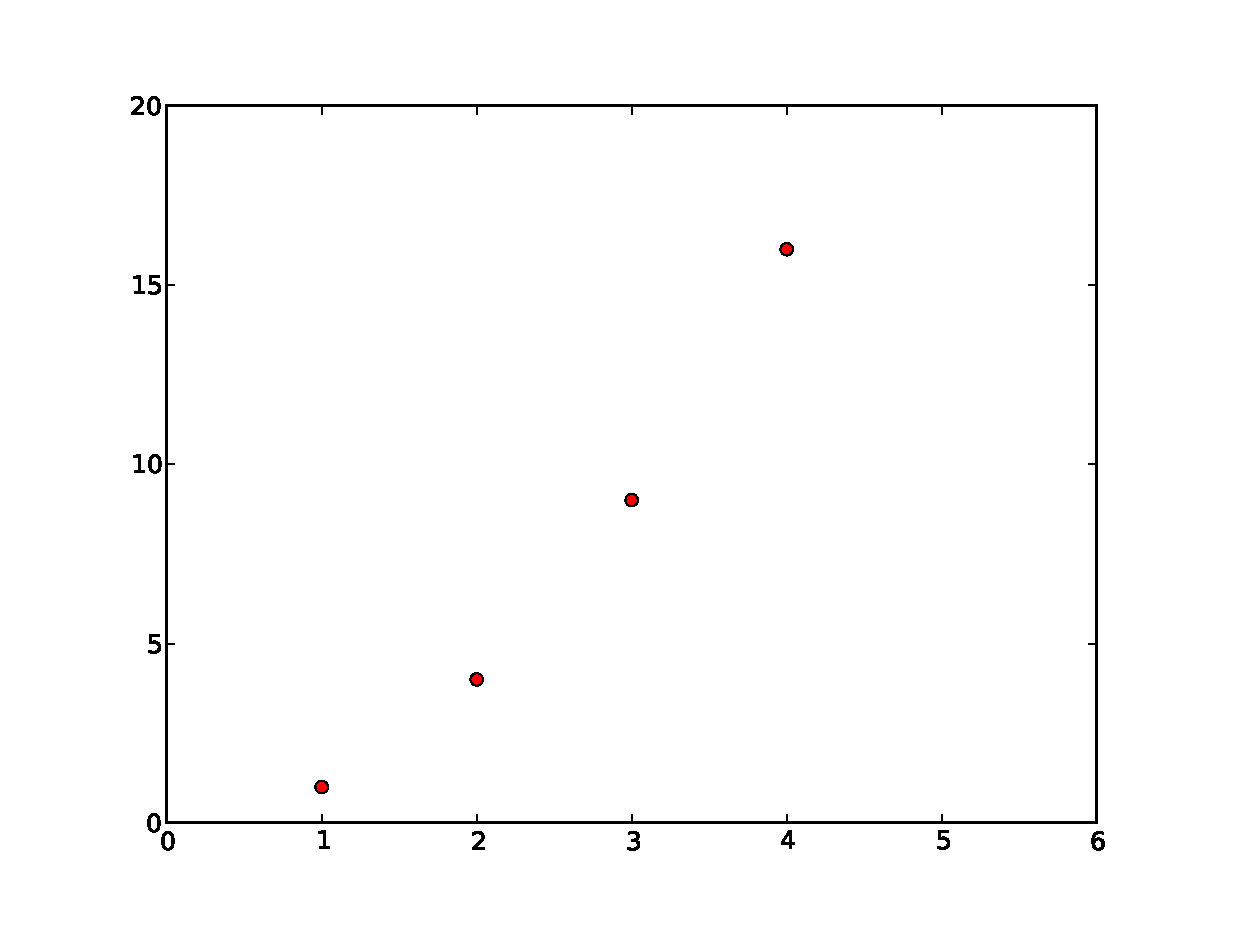
\includegraphics[scale=0.3]{ejemgraf3.eps} 
\end{figure}
\end{minipage}}
\end{frame}
\begin{frame}[fragile]
\frametitle{Ejemplo 4}
\begin{lstlisting}
import numpy as np
import matplotlib.pyplot as plt

t = np.arange(0., 5., 0.2)

# lineas rojas, cuadros azules y triangulos verdes
plt.plot(t, t, 'r--', t, t**2, 'bs', t, t**3, 'g^')
plt.show()
\end{lstlisting}
\end{frame}
\begin{frame}[fragile]
\frametitle{Gr\'{a}fica del Ejemplo 4}
\begin{figure}
	\centering	
	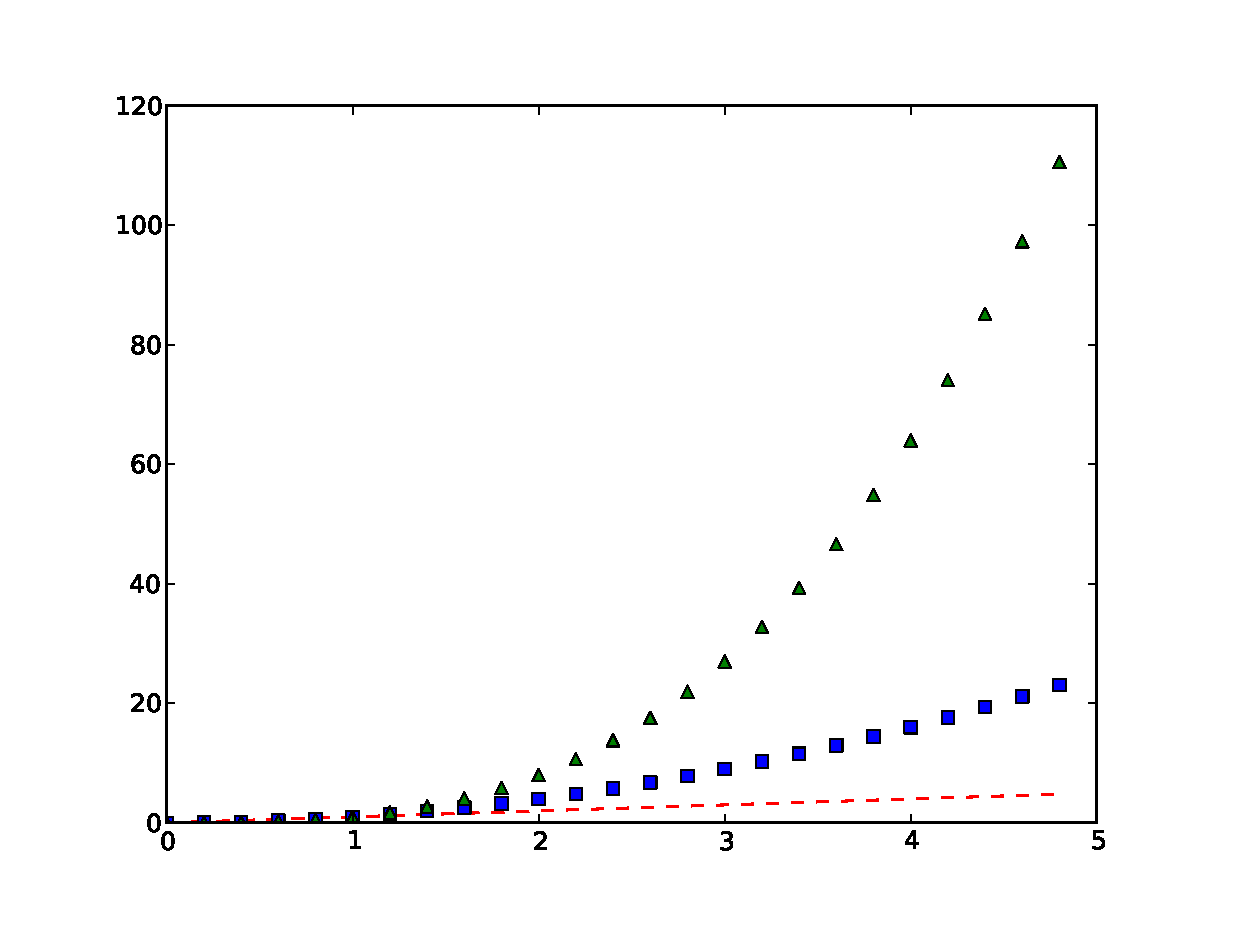
\includegraphics[scale=0.45]{ejemgraf4.eps} 
\end{figure}
\end{frame}
\begin{frame}[fragile]
\frametitle{Ejemplo 5 - M\'{u}ltiples gr\'{a}ficas}
\begin{lstlisting}
import numpy as np
import matplotlib.pyplot as plt

def f(t):
    return np.exp(-t) * np.cos(2*np.pi*t)

t1 = np.arange(0.0, 5.0, 0.1)
t2 = np.arange(0.0, 5.0, 0.02)

plt.figure(1)
plt.subplot(211)
plt.plot(t1, f(t1), 'bo', t2, f(t2), 'k')

plt.subplot(212)
plt.plot(t2, np.cos(2*np.pi*t2), 'r--')
plt.show()
\end{lstlisting}
\end{frame}
\begin{frame}[fragile]
\frametitle{Gr\'{a}fica del Ejemplo 5}
\begin{figure}
	\centering	
	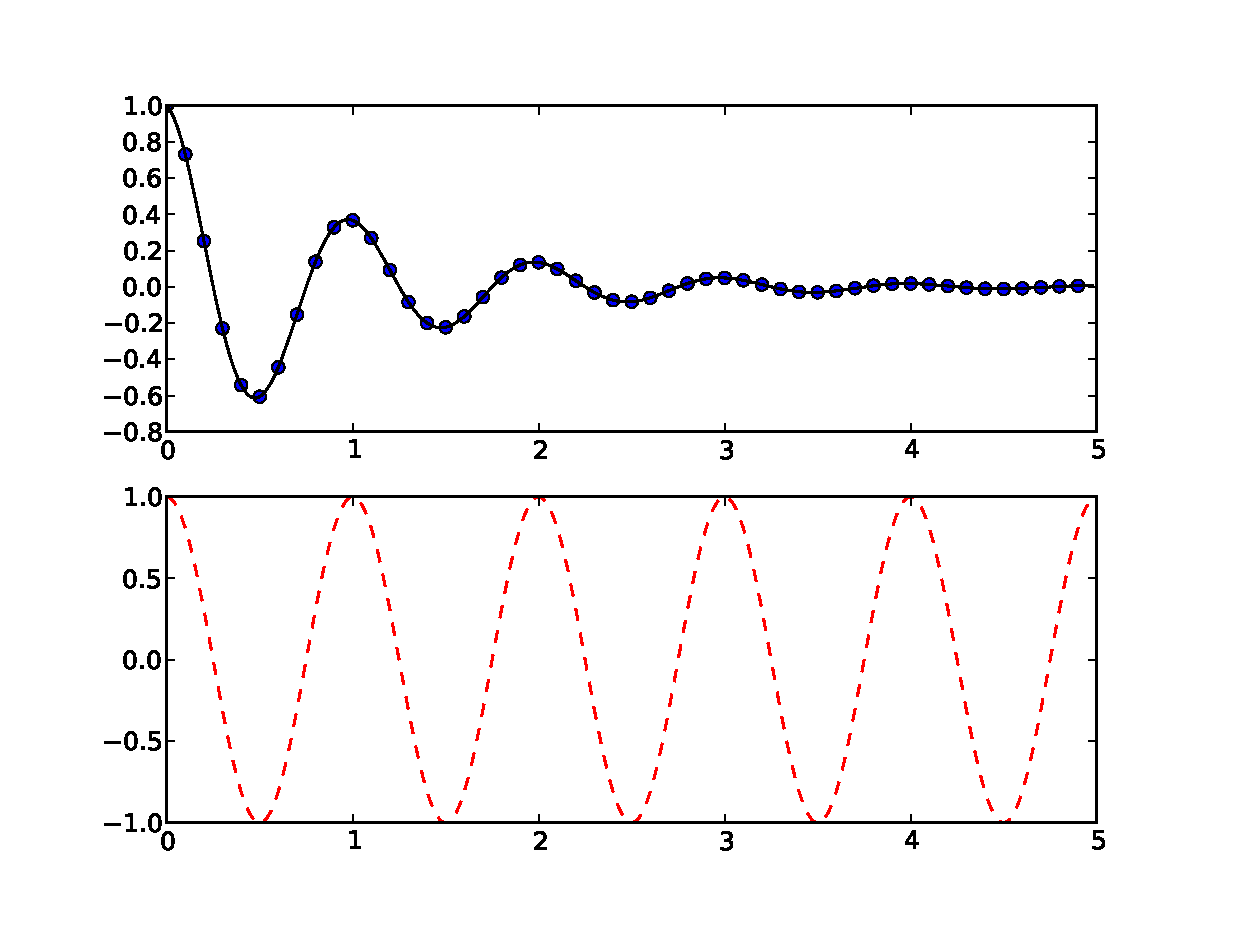
\includegraphics[scale=0.45]{ejemgraf5.eps} 
\end{figure}
\end{frame}
\begin{frame}
\frametitle{Aclaraci\'{o}n sobre m\'{u}ltiples gr\'{a}ficas.}
El comando \texttt{figure} es opcional, ya que \texttt{figure(1)} se genera por defecto, su equivalente es \texttt{subfigure(111)} que se crea tambi\'{e}n por defecto.
\\
\bigskip
El comando \texttt{subplot()} define \texttt{numrows, numcols, fignum}, donde el rango de  \texttt{fignum} var\'{i}a entre 1 y \texttt{numrows*numcols}. Las comas en el comando \texttt{subplot} son opcionales si \texttt{numrows*numcols}$<10$, por lo que es lo mismo \texttt{subplot(211)} y \texttt{subplot(2,1,1)}.
\end{frame}
\begin{frame}[fragile]
\frametitle{Gr\'{a}ficas M\'{u}ltiples}
\begin{figure}
	\centering	
	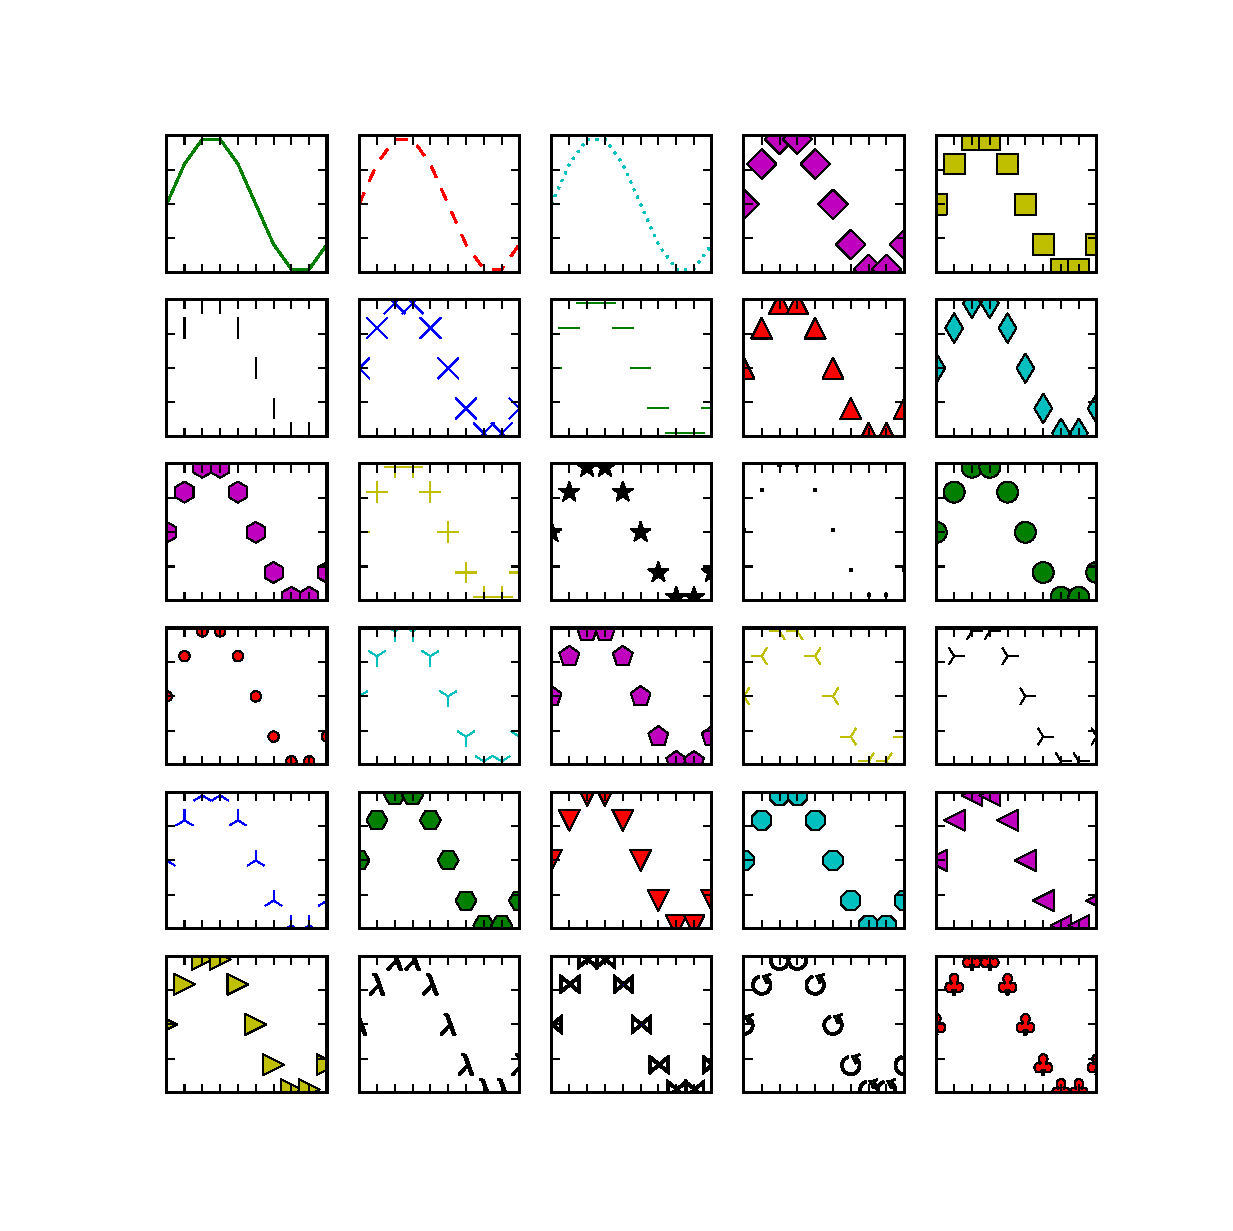
\includegraphics[scale=0.35]{ejemgraf7.eps} 
\end{figure}
\end{frame}
\begin{frame}[fragile]
\frametitle{Ejemplo 6}
\begin{minipage}{0.9\textwidth}
\begin{lstlisting}
#importar Numpy y matplotlib
mu, sigma = 100, 15
x = mu + sigma * np.random.randn(10000)

#el histograma de los datos
n, bins, patches = plt.hist(x, 50, normed=1, facecolor='g', alpha=0.75)

plt.xlabel('Genios')
plt.ylabel('Probabilidad')
plt.title('Histograma de IQ')
plt.text(60, .025, r'$\mu=100,\ \sigma=15$')
plt.axis([40, 160, 0, 0.03])
plt.grid(True)
plt.show()
\end{lstlisting}
\end{minipage}
\end{frame}
\begin{frame}[fragile]
\frametitle{Gr\'{a}fica del Ejemplo 6}
\begin{figure}
	\centering	
	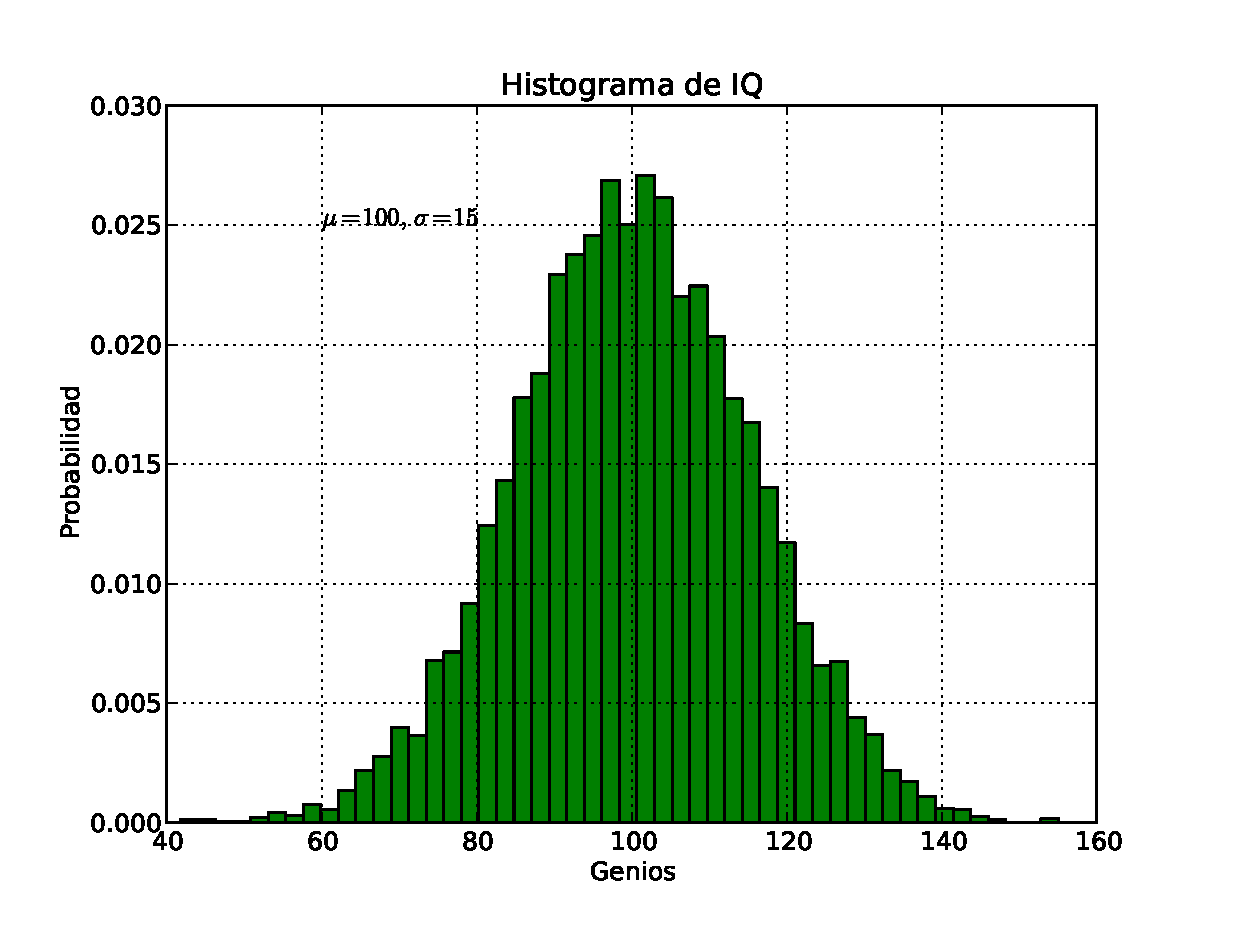
\includegraphics[scale=0.45]{ejemgraf6.eps} 
\end{figure}
\end{frame}
\end{document}